
	For implementing the Particle weighting,  we considered two approaches for comparing the distance measurements from the robot (r) and particles (z):
	
		\begin{enumerate}
			\item Comparing every reading from the sensor individually, so the \textit{posterior} is the product of subtracting each sensor beams as showed on Algorithm 1. 
			\item Comparing the whole vector of readings by adding up the individual readings and then subtracting the scalar number as showed on Algorithm 2:
		\end{enumerate}
	
		\vspace{1em}
		\begin{algorithm}[H]
			\caption{Method 1 for Comparing distance reading} \label{alg:method2}
			... \\
			initialise weigths; \\
			botScan = robot.ultraScan(); \\
			
			\For{$particle \in  particles$} {
				pScan = (particle.ultraScan());\\
				prob=1;\\ 
				\For{$reading \in  particle$} {
					delta =  abs(robotBeamReading - particleBeamReading)\\
					prob = prob * exp( - delta / (2 * sigma*sigma) ) ;}
				weights(i) = prob+damping;}
			...\\
		\end{algorithm}
		\vspace{1em}
			
	
		\vspace{1em}
		\begin{algorithm}[H]
			\caption{Method 1 for Comparing distance reading} \label{alg:method1}
			... \\
			initialise weigths; \\
			botScan = robot.ultraScan(); \\
	 
			\For{$particle \in  particles$} {
				pScan = (particle.ultraScan());\\ 
				delta = sum( abs(pScan - botScan) );\\
				weights(i) = exp( - delta / (2 * sigma * sigma) ) + dampling;}
			...\\
		\end{algorithm}
		\vspace{1em}
	
	We tested both approaches by running the particle filter 500 times on the first map  and measured the convergence time and the distance error. We present the results on (Figure \ref{fig:methods}), we can infer that method one is slightly slower (2.91s vs 2.04s) but more accurate (1.88 cm vs 4.9 cm); however, method 1 is less robust to noisy data since a big difference in one beam can heavily penalise the whole particle, thus we used the method number 2 for further experiments and implementation. 
	

	\begin{figure}[h]
		\centering
		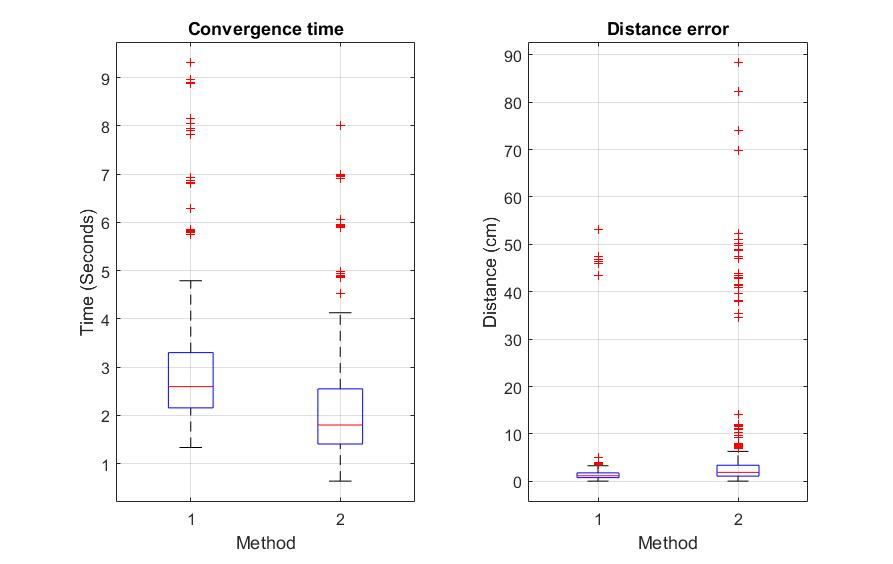
\includegraphics[width=.75\textwidth]{methods}
		\caption{Two approaches for comparing sensor data between the robot and its particles}
		\label{fig:methods}
	\end{figure}
	
	
	
	After finding the optimal number of particles, we aimed for finding an adequate number of beams for the sensor reading towards an accurate and fast implementation.
	
	On the simulation, we let the robot localise itself into the first map and we measured the convergence time of the particle filter and the distance error relative to the actual robot's position, we vary the number of beams from 5 to 40 using increments by 5 and running each experiment 500 times. 
	
	We present the results on (Figure \ref{fig:NumBeams}) and we  inferred that more sensor beams leads to a more accurate pose's estimation but also increases the computational time for convergence since more operations are required. Thus, we select 10 beams as an adequate value since offers both accuracy (mean error of 1.44cm) and fast computation time ( mean 3.34 seconds for convergence).  
	
	\begin{figure}[h]
    \centering
		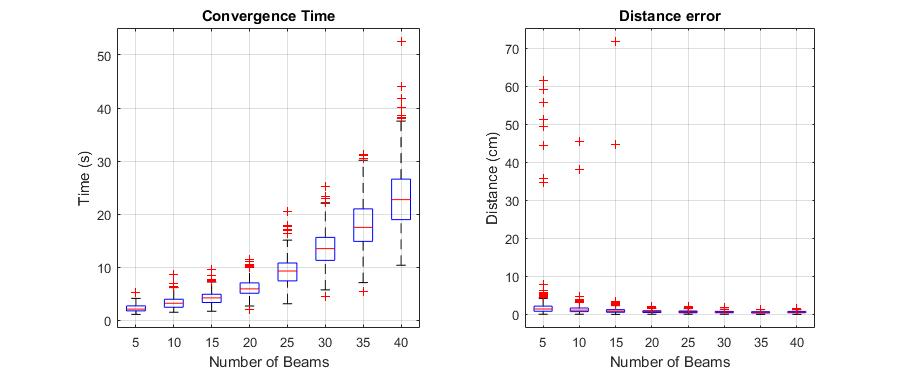
\includegraphics[width=.75\textwidth]{NumberOfBeams}
      \caption{Selecting an adequate number of sensor beams}
    \label{fig:NumBeams}
 	\end{figure}
	
	
	 

	
	